% Main Document File for PhD Proposal
% Urban Heat and Health in Johannesburg: A Multidimensional Analysis of Vulnerability, Explanatory Modelling, and Predictive Outcomes
\documentclass[12pt,a4paper]{article}
\usepackage[utf8]{inputenc}
\usepackage[T1]{fontenc}

% Load newtx packages first without amssymb
\usepackage{newtxtext} % Use Times New Roman instead of times package (matches appendix)
\usepackage{newtxmath} % Times-like math fonts (matches appendix)

% Only load amsmath, not amssymb
\usepackage{amsmath}

\usepackage[margin=2.5cm]{geometry}
\usepackage{setspace}
\usepackage{graphicx}
\graphicspath{{images/}}
\usepackage{booktabs}
\usepackage{tikz}
\usetikzlibrary{arrows.meta,shapes.geometric,shapes.symbols,positioning,fit} % Added libraries for diagrams
\usepackage{natbib}
\usepackage{xcolor}
\usepackage{float}
\usepackage{array}
\usepackage{longtable}
\usepackage{pdflscape}
\usepackage{fancyhdr}
\usepackage{caption}
\usepackage{subcaption}
\usepackage{lastpage} % For total page count
\usepackage{enumitem} % For improved list customization (matches appendix)
\usepackage{hyperref} % Moved to load last to avoid conflicts

% Define version and date information
\newcommand{\protocolversion}{v1.0} % Change this for each new version
\newcommand{\revisiondate}{\today} % This uses today's date, or you can specify a fixed date

% Define colors
\definecolor{witsprimary}{RGB}{0, 87, 164} % Wits University blue
\definecolor{witssecondary}{RGB}{255, 210, 0} % Wits University gold

% Set up headers and footers
\pagestyle{fancy}
\fancyhf{}
\fancyhead[L]{PhD Protocol: Urban Heat and Health in Johannesburg}
\fancyhead[R]{Craig Parker}
\fancyfoot[L]{\small\textit{Version \protocolversion}}
\fancyfoot[C]{\thepage\ of \pageref{LastPage}}
\fancyfoot[R]{\small\textit{Last updated: \revisiondate}}
\renewcommand{\headrulewidth}{0.4pt}
\renewcommand{\footrulewidth}{0.4pt}

% For first page - add version to title page
\fancypagestyle{firstpage}{
    \fancyhf{}
    \fancyfoot[L]{\small\textit{Version \protocolversion}}
    \fancyfoot[C]{\thepage\ of \pageref{LastPage}}
    \fancyfoot[R]{\small\textit{Last updated: \revisiondate}}
    \renewcommand{\headrulewidth}{0pt}
}

% List formatting to match appendix
\setlist{nosep} % Reduce list spacing
\setlist[itemize]{leftmargin=*}
\setlist[enumerate]{leftmargin=*}

% Table formatting to match appendix
\renewcommand{\arraystretch}{1.3} % More space between rows
\newcolumntype{L}[1]{>{\raggedright\arraybackslash}p{#1}} % Left-aligned with width
\newcolumntype{C}[1]{>{\centering\arraybackslash}p{#1}} % Center-aligned with width
\newcolumntype{R}[1]{>{\raggedleft\arraybackslash}p{#1}} % Right-aligned with width

% Caption settings to match appendix
\captionsetup{
  format=plain,
  font=normal,
  labelfont=bf,
  justification=justified,
  singlelinecheck=true
}

% Set headheight to avoid warnings
\setlength{\headheight}{15pt}

% Hyperlink setup - should be last for compatibility reasons
\hypersetup{
    colorlinks=true,
    linkcolor=witsprimary,
    filecolor=witsprimary,
    urlcolor=witsprimary,
    citecolor=witsprimary,
    pdftitle={Urban Heat and Health in Johannesburg: PhD Protocol},
    pdfauthor={Craig Parker},
    pdfsubject={PhD Protocol},
    pdfkeywords={heat, health, climate change, machine learning, vulnerability, Johannesburg}
}

\doublespacing % Double spacing as per guidelines

\begin{document}

% Remove all page numbering for front matter
\pagestyle{empty}
\pagenumbering{gobble}

% Title page
\begin{titlepage}
    \thispagestyle{empty} % Use the special first page style
    \centering
    
\includegraphics[width=0.4\textwidth]{wits_logo.png}\\[1cm]
    
    {\scshape\LARGE University of the Witwatersrand \\
    School of Public Health \par}
    \vspace{1.5cm}
    
    {\huge\bfseries Urban Heat and Health in Johannesburg:\\
    A Multidimensional Analysis of Vulnerability, \\
    Explanatory Modelling, and Predictive Outcomes\par}
    \vspace{1.5cm}
    
    {\large\textit{PhD Protocol}\par}
    \vspace{0.5cm}
    
    {\normalsize\textit{Version \protocolversion}\par} % Version number
    {\normalsize\textit{Last updated: \revisiondate}\par} % Last updated date
    \vspace{0.5cm}
    
    {\large Submitted by:\par}
    {\Large Craig Parker, MSc, MM-PDM, BS\par}
    {\large Wits Planetary Health Research\par}
    \vspace{0.5cm}
    
    {\large Supervisors:\par}
    {\large Dr. Admire Chikandiwa\par}
    {\large Professor Matthew Chersich\par}
    {\large Professor Akbar Waljee\par}
    {\large Dr. Christopher Jack\par}
    \vfill
    
    {\large \today\par}
\end{titlepage}

% Table of contents
\newpage
\pagestyle{empty} % Ensure no numbers on TOC
\tableofcontents
\newpage

% Include the modular sections without forced page breaks
\pagestyle{empty} % Ensure no page numbers on abstract
\section*{Abstract}
\addcontentsline{toc}{section}{Abstract}
This research proposal investigates the complex relationship between urban heat and health in Johannesburg, South Africa. As climate change drives increasing temperatures globally, urban populations face heightened health risks, with vulnerable communities disproportionately affected. 
The study employs a multidimensional approach through three primary objectives: (1) mapping intra-urban heat vulnerability by integrating environmental, socio-economic, and health data; (2) delineating heat-health dynamics through a two-stage explanatory modeling approach that combines hypothesis generation with targeted testing to uncover physiological pathways and temporal effects; and (3) developing a stratified predictive model for heat-related health outcomes.
Drawing on clinical trial data, satellite imagery, climate records, and socioeconomic surveys, this research will apply advanced statistical and machine learning techniques to create vulnerability maps, explain complex relationships, and generate predictive models. The findings aim to inform targeted public health interventions, urban planning decisions, and climate adaptation strategies to protect vulnerable populations from increasing heat exposure in Johannesburg and potentially other African urban centers.

\noindent\rule{\textwidth}{0.5pt}

\vspace{0.5cm}
\noindent\textbf{Keywords:} urban heat, health outcomes, vulnerability mapping, machine learning, climate change, Johannesburg

\section*{Acknowledgements}
\addcontentsline{toc}{section}{Acknowledgements}

This research was conducted as part of the HEat and HEalth African Transdisciplinary (HE²AT) Center initiative, supported by the NIH Common Fund under Award Number U54 TW 012083.
\clearpage

% Start page numbering from introduction (the actual content that counts toward 15 pages)
\pagenumbering{arabic}
\setcounter{page}{1}
\pagestyle{plain} % Ensure page numbers are displayed

% Define a custom page style to ensure numbers appear
\makeatletter
\def\ps@plain{
  \let\@oddhead\@empty
  \def\@oddfoot{\reset@font\hfil\thepage\hfil}
  \let\@evenhead\@empty
  \def\@evenfoot{\reset@font\hfil\thepage\hfil}
}
\makeatother

% Apply the page style
\pagestyle{plain}
\section{Introduction and Background}

\subsection{Climate Change and Heat-Health Impacts in the Johannesburg Context}

Climate change has driven a global temperature increase of over 1.2°C since the Industrial Revolution, with African regions experiencing higher-than-average temperature increases \citep{IPCC2022}. Urban areas are particularly affected due to development patterns and land use changes, with high temperatures increasingly linked to mortality and morbidity, especially during heatwaves \citep{Gasparrini2015, Analitis2018}.

Heat-related risks are rising in Johannesburg at 1753 meters elevation with over 5.87 million inhabitants \citep{Worldometer2023}. The city recorded its highest temperature of 38°C in January 2016, breaking the previous record of 36.5°C from November 2015 \citep{Strydom2016}. Studies show that above a threshold of approximately 18.7°C apparent temperature, all-cause mortality rises by 0.9\% per 1°C increase and by 2.1\% per 1°C among seniors \citep{Wichmann2017, Scovronick2018}. While official records counted only 11 direct heat-related deaths in a recent assessment, researchers estimate the actual heat burden to be much higher \citep{Chersich2023}.

Climate models project substantial warming for Johannesburg. By late-century under a high-emissions scenario, mean annual temperatures in interior South Africa could rise 6--7°C above late 20th-century baselines \citep{Engelbrecht2015}. Even by 2050, Johannesburg may warm by approximately 2°C if global emissions remain high \citep{Engelbrecht2015, Souverijns2022}, with hot nights (minimum temperature >20°C) projected to quadruple from about 10 per year to approximately 40 per year -- and up to 100 in the city's most heat-prone neighbourhoods \citep{WorldBank2024}. Researchers estimate an additional 3--4 weeks of very hot days per year by mid-century \citep{Garland2015}, and the IPCC warns that beyond +2°C of global warming, heat-attributable mortality and morbidity in Africa will sharply rise \citep{IPCC2022}.

\subsection{Socio-Spatial Inequity and Heat Vulnerability}

Johannesburg's subtropical highland climate features hot summer days (October-April), often with afternoon thundershowers, and dry, sunny winter days with cold nights (May-September) \citep{Tyson2000}. However, the city's socio-spatial layout -- largely a legacy of apartheid-era planning -- significantly shapes heat vulnerability patterns today. Historically, policies created wealthy, low-density suburbs with ample green spaces alongside dense townships with minimal vegetation or services \citep{Giombini2022, Venter2020}. This has resulted in stark contrasts in urban heat exposure, with lush neighbourhoods enjoying cooler microclimates, while nearby townships can be approximately 6°C hotter than the surrounding countryside \citep{WorldBank2024, Habitat2023}.

Housing quality differences further exacerbate exposure: informal housing can become significantly hotter, with indoor temperatures up to 15°C higher than in modern housing during the day \citep{Naicker2017}. Apartheid geography has effectively embedded vulnerability into Johannesburg's landscape, clustering heat risk in marginalized communities \citep{Strauss2019}.

\subsection{Conceptual Framework and Research Gaps}

This research employs a comprehensive framework for heat vulnerability encompassing three interconnected dimensions: exposure, sensitivity, and adaptive capacity \citep{IPCC2022}:

\begin{itemize}
    \item \textit{Exposure} refers to heat stress degree and duration, with dense urban areas showing significantly higher surface temperatures (up to 5°C) compared to well-vegetated neighbourhoods \citep{Li2017, Santamouris2015}.
    
    \item \textit{Sensitivity} reflects population susceptibility influenced by socio-economic conditions and health status, with chronic conditions significantly increasing heat-related health risks \citep{Watts2023, Khosla2021, Souverijns2022}.
    
    \item \textit{Adaptive capacity} depends on access to healthcare, cooling infrastructure, and social support systems \citep{Ansah2024}, with limited access to healthcare affecting vulnerability to heat, as demonstrated by increased heat-related mortality in areas with restricted medical services \citep{Murage2020}.
\end{itemize}

Despite growing climate health research worldwide, significant gaps remain in understanding the dynamics of heat health in urban African contexts. Most existing studies focus on high-income regions, overlooking the distinct characteristics of African cities \citep{Khine2023, Pasquini2020}. Key limitations include:

\begin{enumerate}
    \item \textbf{Scarcity of African Urban Heat-Health Studies:} Limited research examining the impacts of heat on health in African urban settings hinders the development of region-specific interventions \citep{Ncongwane2021, Wright2019}.

    \item \textbf{Siloed Disciplinary Approaches:} Lack of interdisciplinary collaboration results in fragmented insights that fail to capture the multifaceted nature of heat-health challenges \citep{Jack}.

    \item \textbf{Unique Urban Challenges:} African cities face distinct issues stemming from historical development patterns, unique disease profiles, and diverse urban morphologies requiring tailored research approaches \citep{Giombini2022, Venter2020}.
\end{enumerate}

Johannesburg exemplifies these challenges through its historical development and urban disparities \citep{Strauss2019}, high disease burden from both communicable and non-communicable diseases \citep{Wright2021}, and accelerated warming projections \citep{Engelbrecht2015, Souverijns2022}. Addressing these gaps is crucial for developing heat health strategies tailored to African urban contexts.

\section{Aims and Objectives}
% Load graphicx package in preamble if not already loaded
\graphicspath{{./images/}}

\subsection{Primary Aim}
This research aims to deepen our understanding of spatially and demographically stratified heat-health interactions in Johannesburg, developing evidence-based approaches to mitigate health risks from rising urban temperatures. By examining the complex interplay between urban heat, socioeconomic factors, and health outcomes, this project seeks to bridge critical knowledge gaps in urban climate-health research within the African context, with potential applications for similar urban environments globally.

\subsection{Specific Objectives}
This research is structured around three interconnected objectives that progress from descriptive analysis to explanatory insights and ultimately to predictive capabilities:

\subsubsection{Objective 1: Intra-urban Heat Vulnerability Mapping}
The first objective centres on comprehensive spatial vulnerability assessment to identify patterns of heat risk across Johannesburg's diverse urban landscape. This mapping process will examine how historical urban development patterns, particularly those influenced by apartheid-era planning, continue to shape contemporary heat vulnerability. Through this assessment, we will identify priority intervention areas and quantify multidimensional vulnerability patterns with particular emphasis on socio-spatial inequities. This objective will result in detailed vulnerability characterization that can directly inform targeted urban planning and public health interventions.

\subsubsection{Objective 2: Heat-Health Dynamics Exploration}
Building on the vulnerability assessment, the second objective aims to unravel complex heat-health relationships by investigating the underlying physiological mechanisms through which heat exposure affects human health. Through a two-stage modelling approach, we will first generate hypotheses about key physiological pathways and then systematically test these hypotheses using targeted feature engineering. This component will focus particularly on metabolic, renal, and inflammatory responses to heat stress, examining how these systems interact across multiple temporal scales. 

The research will explore non-linear climate-health interactions across different temperature thresholds while distinguishing between immediate (0-24 hours), short-term (1-7 days), and medium-term (7-30 days) physiological effects. By applying interpretable machine learning techniques with clinically validated pathway diagrams, we seek to establish causal mechanisms that explain differential vulnerability between population groups and identify critical intervention points for health protection during heat events. This explanatory approach moves beyond simple statistical associations to provide mechanistic insights to inform targeted clinical and public health responses.

\subsubsection{Objective 3: Stratified Heat-Health Prediction Modeling}
The final objective leverages insights from the previous components to develop predictive frameworks for heat-related health outcomes in Johannesburg. These predictive capabilities will be stratified both geographically and demographically to account for differential vulnerability across the city's diverse population. The objective seeks to identify specific risk conditions at various temperature thresholds, enabling the development of targeted early warning systems. Special attention will be given to demographic-specific risk stratification for vulnerable populations, including the elderly, those with pre-existing conditions, and communities with limited adaptive capacity. The resulting predictive tools will provide actionable intelligence for healthcare systems and emergency response planning.

\begin{figure}[h]
    \centering
    % Adding a white background rectangle to prevent text showing through
    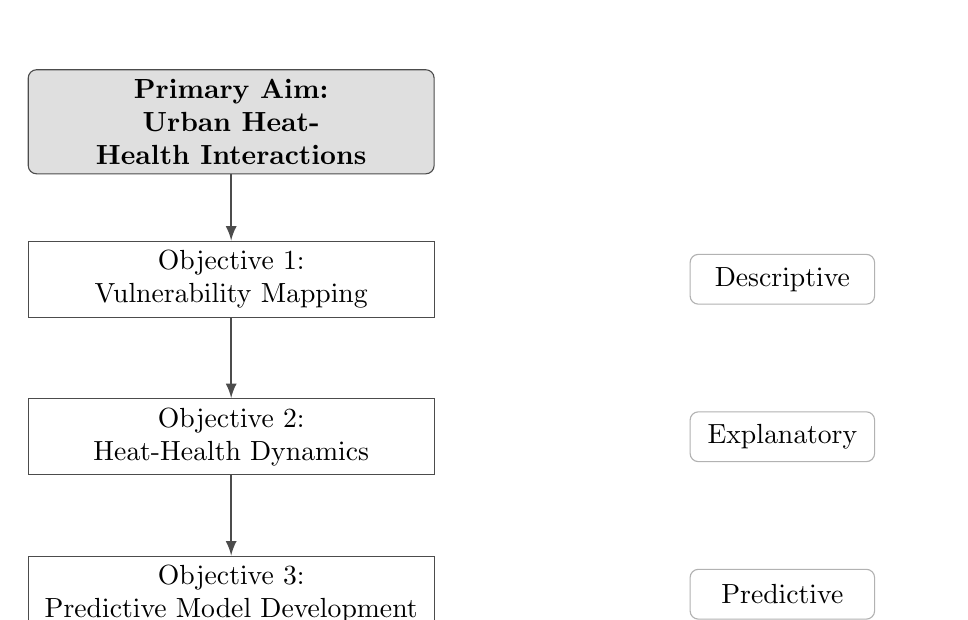
\begin{tikzpicture}[
        block/.style={rectangle, draw, rounded corners=3pt, text width=14em, text centered, minimum height=2.5em, font=\bfseries, fill=gray!15, draw=black!70},
        objective/.style={rectangle, draw, text width=14em, text centered, minimum height=2.5em, draw=black!70},
        arrow/.style={thick,->,>=stealth, draw=black!70},
        label/.style={rectangle, draw, rounded corners=3pt, fill=white, text width=6em, text centered, minimum height=1.8em, draw=black!30}
    ]
    
    % Add background rectangle to prevent text showing through
    \fill[white] (-1,-6.5) rectangle (9,0.5);
    
    % Primary Aim block with darker fill
    \node[block, fill=gray!25] (aim) at (0,0) {Primary Aim:\\Urban Heat-Health Interactions};
    
    % Objectives with distinctive styling
    \node[objective, fill=white] (obj1) at (0,-2) {Objective 1:\\Vulnerability Mapping};
    \node[objective, fill=white] (obj2) at (0,-4) {Objective 2:\\Heat-Health Dynamics};
    \node[objective, fill=white] (obj3) at (0,-6) {Objective 3:\\Predictive Model Development};
    
    % Arrows with slight curve for visual interest
    \draw[arrow, -latex] (aim) -- (obj1);
    \draw[arrow, -latex] (obj1) -- (obj2);
    \draw[arrow, -latex] (obj2) -- (obj3);
    
    % Labels with better positioning and styling
    \node[label] at (7,-2) {Descriptive};
    \node[label] at (7,-4) {Explanatory};
    \node[label] at (7,-6) {Predictive};
    
    \end{tikzpicture}
    \caption{Hierarchical framework of research objectives showing progression from descriptive to predictive approaches.}
    \label{fig:aims_objectives}
\end{figure}

Together, these three objectives form an integrated research framework that addresses the spatial dimension (identifying vulnerable areas), the physiological dimension (understanding underlying mechanisms), and the temporal dimension (developing predictive capabilities). This multi-dimensional approach will provide a comprehensive understanding of heat-health interactions in Johannesburg, with implications for urban planning, public health interventions, and climate adaptation strategies. The research design intentionally builds each objective upon the findings of the previous one, creating a cohesive analytical pathway from vulnerability characterization to mechanistic understanding to practical solution development. This progression from descriptive to explanatory to predictive aims reflects the holistic nature of the heat-health challenge and enables development of targeted, evidence-based interventions.

\section{Methodology}

\subsection{Study Design}
This study employs a mixed-methods design integrating quantitative geospatial analysis with qualitative community-engaged research across three primary phases:
\begin{enumerate}
    \item \textbf{Vulnerability Mapping} - Developing geographically weighted heat vulnerability indices
    \item \textbf{Causal Analysis} - Identifying key causal pathways and mechanisms
    \item \textbf{Predictive Modeling} - Developing heat-health forecasting capabilities
\end{enumerate}

While the findings from these three phases will generate insights that could inform future intervention strategies and policy recommendations, the actual development and implementation of such interventions falls outside the scope of this PhD project.

\subsection{Data Sources and Collection}
Health data spanning 2000--2022 will be drawn from clinical trials and cohort studies conducted in Johannesburg that meet defined inclusion criteria: cohorts or trials with 200 adult participants, prospectively collected data, comprehensive clinical and laboratory variables, and appropriate ethics approvals. The dataset will include clinical indicators and laboratory tests covering renal, metabolic and inflammatory markers and demographic/socioeconomic factors. 

To address the significant impact of COVID-19 on both healthcare utilization patterns and population vulnerability, 2020--2022 data will undergo specialized analytical treatment, including: (1) stratified analysis by pandemic periods (pre-pandemic, peak waves, inter-wave periods); (2) adjustment for documented disruptions in healthcare-seeking behavior; and (3) incorporation of COVID-19 case and mortality data as potential confounding or effect-modifying variables. Changes in vulnerability patterns during this period will be explicitly modeled to understand how the pandemic may have altered underlying vulnerability dynamics. A comprehensive overview of all data sources is provided in Appendix Table 1.

\subsubsection{Environmental and Socioeconomic Data}
Environmental parameters will be derived from multiple validated sources, including Landsat 8 \citep{landsat8}, Sentinel-2 \citep{sentinel2}, ERA5 reanalysis \citep{era5}, and the Copernicus Climate Data Store \citep{copernicus_climate_data_store}. These data streams will provide high-resolution measurements of Land Surface Temperature, vegetation indices, air temperature, and derived heat metrics. Socioeconomic determinants will be incorporated through ward-level data from the Gauteng City-Region Observatory Quality of Life Surveys \citep{gcro_qol_survey}, capturing housing quality, infrastructure adequacy, and healthcare access. The data processing and integration workflow is detailed in Appendix Table 2, with specific security measures outlined in Appendix Table 3.

\subsubsection{Health and Socioeconomic Data}
We will integrate: daily mortality records and hospital admission data (with focus on cardiovascular, respiratory, and heat-specific diagnoses), demographic variables from Statistics South Africa, social vulnerability indicators (housing quality, utility access), pre-existing health condition prevalence, and COVID-19 data to assess potential interactive effects with heat vulnerability. 

A key methodological challenge is capturing vulnerability in Johannesburg's mixed socioeconomic areas where informal settlements often exist adjacent to middle and high-income neighborhoods. To address this, we will implement: (1) sub-ward level analysis where data resolution permits; (2) heterogeneity analysis within administrative units using variance metrics; and (3) mixed-effects models that explicitly account for within-ward socioeconomic variation. This approach will enable identification of vulnerable populations that might otherwise be masked by ward-level aggregation in socioeconomically heterogeneous areas. All datasets will be harmonized to comparable spatial units for integrated analysis, with explicit documentation of data quality metrics for each source.

\subsubsection{Sample Size Justification}
The study's statistical power is ensured through comprehensive data coverage and adequate sample sizes. For vulnerability mapping, data from all 135 wards provide complete spatial coverage. For the explanatory and predictive modelling components, the combined dataset of approximately 5,000--7,000 records substantially exceeds the minimum requirement of 10-20 observations per predictive feature (with 20-25 features anticipated). This sample size provides >80\% power to detect clinically meaningful effects, calculated as:

\begin{equation}
n = \frac{2(Z_{\alpha/2} + Z_{\beta})^2\sigma^2}{\Delta^2}
\end{equation}

where $Z_{\alpha/2}$ and $Z_{\beta}$ are standard normal deviates for type I and II errors, $\sigma^2$ is the expected variance, and $\Delta$ is the minimal detectable effect size.

\subsection{Analytical Approaches}

\subsubsection{Geographically Weighted Vulnerability Mapping}\label{gwpca}
A key innovation in this study is the application of Geographically Weighted Principal Component Analysis (GWPCA), which accounts for spatially heterogeneous relationships between vulnerability indicators \citep{Quispe2023, Praharaj2024}. This is crucial in Johannesburg given its extreme socio-spatial fragmentation. The GWPCA approach includes: (1) indicator selection across exposure, sensitivity, and adaptive capacity domains; (2) spatial bandwidth optimization through cross-validation; (3) local component extraction allowing vulnerability factors to vary spatially; (4) construction of location-specific vulnerability indices; (5) spatial mapping; and (6) comparative analysis between global and local statistical approaches. Implementation will utilize the GWmodel package in R.

\subsubsection{Causal Machine Learning Approaches}
To move beyond correlation and identify causal mechanisms linking urban form, socioeconomic conditions, and heat-health outcomes, we will employ: (1) causal structure learning using the PC algorithm to discover potential causal relationships; (2) causal effect estimation using double machine learning and causal forests to estimate heterogeneous treatment effects of specific urban features; and (3) causal mediation analysis to quantify direct and indirect pathways through which urban characteristics influence health outcomes. Implementation will use causal-learn and econml Python packages, with sensitivity analyses to assess robustness.

\subsection{Objective 1: Vulnerability Mapping}
Geospatial data will undergo rigorous preprocessing, including normalization, completeness assessments, and spatial harmonization. The methodology employs Geographically Weighted Principal Component Analysis (GWPCA) \citep{Harris2011, Quispe2023} to develop a comprehensive Heat Vulnerability Index that accounts for spatial non-stationarity in vulnerability relationships.

\subsection{Objective 2: Explanatory Modeling}
The explanatory modelling framework employs a two-stage clinical-computational approach examining both physiological pathways and temporal effects of heat exposure. This framework harmonizes data from multiple cohort studies to investigate underlying mechanisms across different physiological systems.

\subsubsection{Clinical Pathway Validation}
Working with clinical experts, we will develop comprehensive physiological pathway diagrams representing hypothesized heat-health mechanisms at multiple biological levels. These diagrams will be rigorously validated through expert consensus panels and systematic literature review, establishing physiologically plausible causal pathways before computational analysis.

\subsubsection{Temporal Heat Exposure Modeling}
To capture the dynamic nature of heat exposure, we will develop spatiotemporal models that characterize: (1) diurnal patterns of day-night temperature variations; (2) seasonal variations between summer and winter; (3) extreme heat events and their spatiotemporal distributions; and (4) long-term trends under climate change scenarios. These analyses will employ time series modeling, extreme value theory, and climate downscaling approaches.

\subsection{Objective 3: Predictive Modeling}
The predictive framework integrates environmental, socioeconomic, and health data to forecast heat-related health outcomes within a 24--72 hour horizon. The methodology employs advanced feature engineering combining domain knowledge with statistical selection techniques including mutual information analysis and recursive feature elimination with cross-validation to identify optimal predictive variables while controlling for collinearity.

Rather than relying on a single algorithm, the approach employs a carefully calibrated ensemble that combines gradient boosting methods, random forests, and other algorithms through a meta-learning framework. For the gradient boosting component, the objective function being optimized is:

\begin{equation}
\mathcal{L}(\phi) = \sum^n_{i=1} l(y_i, \hat{y}_i) + \sum^K_{k=1} \Omega(f_k)
\end{equation}

where $l$ is the loss function comparing the prediction $\hat{y}_i$ with the target $y_i$, and $\Omega$ represents the regularization term controlling model complexity.

The validation strategy employs forward-chaining time-series cross-validation to realistically simulate forecasting scenarios, with performance evaluated using metrics including area under the receiver operating characteristic curve (AUC-ROC):

\subsubsection{Model Accuracy and Reliability Measures}
To ensure predictive model accuracy and reliability, particularly across Johannesburg's diverse urban contexts, we will implement a comprehensive validation framework. This includes: (1) spatially stratified cross-validation to test model performance across different urban morphologies; (2) out-of-distribution detection methods to identify and address anomalous predictions; (3) uncertainty quantification through conformal prediction intervals; and (4) regular recalibration procedures to maintain model accuracy over time. 

Our model evaluation will employ metrics beyond traditional accuracy measures (AUC-ROC, F1) to include reliability diagrams, expected calibration error, and variable-specific sensitivity analyses. This approach ensures that predictions remain valid across the city's diverse built environments and socioeconomic contexts, with explicit reliability assessments for informal settlements and areas undergoing rapid urban transformation.

\subsubsection{Data Quality Variability Management}
A critical challenge in urban vulnerability modeling is the heterogeneous quality of data across sources and locations. To address this issue comprehensively, we will implement:

\begin{enumerate}
    \item \textbf{Quality-weighted modeling}: All data sources will be assigned quality scores based on completeness, consistency with reference sources, and temporal coverage. These scores will be incorporated into model weights, reducing the influence of lower-quality data on final predictions.
    
    \item \textbf{Spatial quality correction}: For areas with known data quality issues (particularly informal settlements with limited administrative data), we will implement targeted correction factors derived from community-based validation exercises.
    
    \item \textbf{Ensemble methods for uncertainty quantification}: By combining multiple modeling approaches with different sensitivity to data quality issues, we will generate robust confidence intervals that reflect true prediction uncertainty.
    
    \item \textbf{Temporal stability analysis}: We will explicitly test how vulnerability patterns have changed over the 20-year study period, with particular attention to informal settlement growth areas and regions undergoing significant urban transformation.
\end{enumerate}

These approaches directly address concerns about varying data quality across Johannesburg's diverse urban contexts and ensure that model outputs appropriately reflect underlying confidence levels, particularly in areas where traditional data collection faces significant challenges.

\subsection{Forecast Window Selection}
The 24--72 hour forecast window was selected based on three key considerations. First, physiological evidence indicates that significant heat-health impacts manifest within 1-3 days of exposure \citep{Gasparrini2015, Kinney2020}, making this the critical intervention window for preventative healthcare measures. Second, meteorological forecast accuracy significantly degrades beyond 72 hours, particularly for urban microclimates, limiting the actionable reliability of longer-term predictions. Third, stakeholder consultations with healthcare providers indicated that a 1-3 day window optimally balances advance warning with operational response capabilities in Johannesburg's healthcare system. Sensitivity analysis will test alternative windows (12--24 hours and 72--120 hours) to assess the stability of predictive relationships across different temporal scales.

\begin{equation}
\text{AUC-ROC} = \int^1_0 TPR(FPR^{-1}(t))dt
\end{equation}

where $TPR$ is the true positive rate and $FPR$ is the false positive rate at different classification thresholds.

The modelling output translates into actionable intelligence through stratified risk profiles, geospatial risk mapping, and population-specific threshold recommendations. This translation from statistical prediction to practical application ensures research findings can directly inform heat-health interventions and resource allocation for vulnerable populations in Johannesburg.

\section{Ethical Considerations}

This study received ethical approval from the Wits Human Research Ethics Committee (reference 220606) and complies with U.S. Department of Health and Human Services regulations (45 CFR 46). Privacy protection includes data minimization, secure servers with restricted access, and geographical jittering/aggregation in compliance with South Africa's Protection of Personal Information Act (POPIA, 2013).

For secondary data usage, contractual guarantees from data providers confirm appropriate consent practices. Ethical risks—such as re-identification, secondary consent issues, and community stigmatization—are mitigated through data aggregation, secure storage, broad consent waivers, and responsible community engagement.

Detailed POPIA compliance framework and data protection procedures are provided in Appendix B.

\section{Expected Outcomes and Impact}

\subsection{Research Outputs}
This doctoral research will generate several significant outputs, including a spatially explicit heat vulnerability index for Johannesburg, a comprehensive explanatory model of urban heat-health relationships, and a validated predictive framework for heat-health outcomes under varied climate scenarios. The work will also produce evidence-based policy recommendations for city planning and public health systems, culminating in at least three peer-reviewed publications addressing vulnerability mapping, explanatory modelling, and predictive applications.

\subsection{Anticipated Impact}
The research is expected to yield significant impacts by enhancing understanding of fine-scale spatial patterns of heat vulnerability in Johannesburg, improving heat-health early warning systems, and identifying priority areas for targeted intervention. This will enable more efficient resource allocation and provide robust, evidence-based policy guidance for urban heat adaptation, particularly for informal settlements and densely populated areas. These methodological advances in integrated urban heat health research can be adapted for other African urban contexts.

\subsection{Knowledge Translation}
Research findings will be strategically disseminated through peer-reviewed publications in journals spanning public health, climate science, and urban planning disciplines. Additional dissemination channels include presentations at national and international conferences, targeted policy briefs for local and national authorities, community engagement workshops in vulnerable areas, and interactive data visualization tools to facilitate stakeholder decision-making. Detailed impact assessment metrics and comprehensive dissemination strategies are provided in Appendix D.

% Project Timeline Section
\section{Project Timeline}
This 36-month PhD research will progress through four key phases, with critical milestones at months 3 (M1: protocol finalization), 9 (M2: data acquisition completion), 18 (M3: vulnerability mapping), and 30 (M4: model validation), culminating in thesis submission at month 36.

The research timeline includes four major publications: a protocol paper titled ``Leveraging data science and machine learning for urban climate adaptation in two major African cities: a HE2AT Center study protocol'' \cite{Jack} (Month 4), followed by three objective-specific publications: ``Quantifying intra-urban socio-economic and environmental vulnerability to extreme heat events in Johannesburg, South Africa'' (Month 9), ``Uncovering Heat-Health Pathways in Johannesburg: An Explanatory Machine Learning Approach Using Harmonized Urban Cohort Data'' (Month 19), and ``Developing Stratified Heat-Health Early Warning Systems for Johannesburg: Integration of Vulnerability Mapping and Predictive Modeling'' (Month 33).
Primary risks include data accessibility challenges, computational constraints, and model performance issues. Detailed timelines, activities, and risk mitigation strategies are provided in Appendix C.

\section{Supervision}

This research will be conducted under the guidance of a multidisciplinary supervisory team with expertise spanning clinical epidemiology, public health, statistical modeling, and climate science. The team includes Dr. Admire Chikandiwa (Wits University), Professor Matthew Chersich (Trinity College/Wits University), Professor Akbar Waljee (University of Michigan), and Dr. Christopher Jack (University of Cape Town).

Monthly progress meetings and bi-weekly consultations will ensure consistent guidance throughout the research process. A detailed supervision framework, including supervisor profiles and advisory committee information, is provided in Appendix E.

% Stop page numbering for references
\clearpage
\pagestyle{empty}
\pagenumbering{gobble}
\makeatletter
\def\@oddfoot{}
\def\@evenfoot{}
\makeatother
\section{References}

\bibliographystyle{apalike}
\bibliography{references}

% Note: The actual references will be generated from the references.bib file.
% Below is a sample of references that would be included in that file:

% @article{Gasparrini2015,
%   title={Mortality risk attributable to high and low ambient temperature: a multicountry observational study},
%   author={Gasparrini, Antonio and Guo, Yuming and Hashizume, Masahiro and Lavigne, Eric and Zanobetti, Antonella and Schwartz, Joel and Tobias, Aurelio and Tong, Shilu and Rocklöv, Joacim and Forsberg, Bertil and others},
%   journal={The Lancet},
%   volume={386},
%   number={9991},
%   pages={369--375},
%   year={2015},
%   publisher={Elsevier}
% }
% 
% @article{Analitis2018,
%   title={Synergistic effects of ambient temperature and air pollution on health in Europe: results from the PHASE project},
%   author={Analitis, Antonis and De' Donato, Francesca and Scortichini, Matteo and Lanki, Timo and Basagana, Xavier and Ballester, Ferran and Astrom, Christofer and Paldy, Anna and Pascal, Mathilde and Gasparrini, Antonio and others},
%   journal={International journal of environmental research and public health},
%   volume={15},
%   number={9},
%   pages={1856},
%   year={2018},
%   publisher={MDPI}
% }
% 
% @article{Scovronick2018,
%   title={The association between ambient temperature and mortality in South Africa: A time-series analysis},
%   author={Scovronick, Noah and Sera, Francesco and Acquaotta, Fiorella and Garzena, Diego and Fratianni, Simona and Wright, Caradee Y and Gasparrini, Antonio},
%   journal={Environmental research},
%   volume={161},
%   pages={229--235},
%   year={2018},
%   publisher={Elsevier}
% }
% 
% @article{Wichmann2017,
%   title={Heat effects of ambient apparent temperature on all-cause mortality in Cape Town, Durban and Johannesburg, South Africa: 2006-2010},
%   author={Wichmann, Janine},
%   journal={Science of the Total Environment},
%   volume={587},
%   pages={266--272},
%   year={2017},
%   publisher={Elsevier}
% }
% 
% @book{Tyson2000,
%   title={Weather and climate of southern Africa},
%   author={Tyson, Peter D and Preston-Whyte, Robert A},
%   year={2000},
%   publisher={Oxford University Press}
% }
% 
% @article{Venter2020,
%   title={Green Apartheid: Urban green infrastructure remains unequally distributed across income and race geographies in South Africa},
%   author={Venter, Zander S and Shackleton, Charlie M and Van Staden, Francini and Selomane, Odirilwe and Masterson, Vanessa A},
%   journal={Landscape and Urban Planning},
%   volume={203},
%   pages={103889},
%   year={2020},
%   publisher={Elsevier}
% }
% 
% @article{Chen2023,
%   title={Rising vulnerability of compound risk inequality to ageing and extreme heatwave exposure in global cities},
%   author={Chen, Mengqiao and Barton, Jennifer E and Headen, Ian and Green, Christine and Holland, Greg J and Lin, Bonnie B},
%   journal={npj Urban Sustainability},
%   volume={3},
%   number={1},
%   pages={38},
%   year={2023},
%   publisher={Nature Publishing Group UK London}
% }
% 
% @article{Khine2023,
%   title={The Implications of Climate Change on Health among Vulnerable Populations in South Africa: A Systematic Review},
%   author={Khine, May Myat and Langkulsen, Uma},
%   journal={International Journal of Environmental Research and Public Health},
%   volume={20},
%   number={4},
%   pages={3468},
%   year={2023},
%   publisher={MDPI}
% }
% 
% @article{Jack2024,
%   title={Leveraging data science and machine learning for urban climate adaptation in two major African cities: a HE²AT Center study protocol},
%   author={Jack, Christopher and Parker, Craig and Kouakou, Yao Etienne and Joubert, Bonnie and McAllister, Kimberly A and Ilias, Maliha and Maimela, Gloria and Chersich, Matthew and Makhanya, Sibusisiwe and Luchters, Stanley and others},
%   journal={BMJ open},
%   volume={14},
%   number={1},
%   pages={e077529},
%   year={2024},
%   publisher={British Medical Journal Publishing Group}
% }
% 
% @misc{Worldometer2023,
%   title={World population by country},
%   author={Worldometer},
%   year={2023},
%   note={Retrieved from \url{https://www.worldometers.info/world-population/population-by-country/}}
% }
% 
% @misc{CityOfJohannesburg2021,
%   title={Climate Action Plan City Of Johannesburg},
%   author={{City of Johannesburg}},
%   year={2021},
%   note={Retrieved from \url{https://joburg.org.za/documents\_/Documents/City\%20of\%20Johannesburg\%20-\%20Climate\%20Action\%20Plan\%20\%28CAP\%29.pdf}}
% }

% Clear note about appendices being in a separate document
% Clear note about appendices being in a separate document
\newpage
\section*{Appendices}
\begin{center}
\large\textbf{NOTE:} \\
\normalsize
All appendices and supplementary tables are provided in a separate document titled:\\
\textit{"Appendices: Data Management and Methodological Tables for PhD Proposal"}\\
\vspace{0.5cm}
This separation has been implemented to comply with page count requirements.\\
\vspace{0.5cm}
The appendix document includes:
\end{center}

\begin{itemize}[leftmargin=*, itemsep=0.3em]
    \item \textbf{Appendix F: Supplementary Figures}
    \begin{itemize}[leftmargin=*]
        \item F.1 Project Framework: Heat Vulnerability Assessment
        \item F.2 Maximum Temperature Distribution
        \item F.3 Seasonal Heat Pattern Analysis
        \item F.4 Global Temperature Trends
        \item F.5 Urban Heat Stress Patterns
        \item F.6 Heat Vulnerability Index Components
        \item F.7 Heat-Health Mechanisms Pathways
        \item F.8 Data Sources and Integration Framework
    \end{itemize}
    
    \item \textbf{Data Management and Methodological Tables}
    \begin{itemize}[leftmargin=*]
        \item Table 1: Key Data Sources for Heat-Health Research
        \item Table 2: Data Processing and Integration Workflow
        \item Table 3: Data Access Levels and Security Measures
        \item Table 4: Geographic De-identification Techniques
        \item Table 5: Data Request and Approval Process
        \item Table 6: Methodological Approaches for Research Objectives
        \item Table 7: Time-Lag Analysis of Heat-Health Effects
    \end{itemize}
    
    \item \textbf{Appendix A:} Roles and Responsibilities in Data Management
    
    \item \textbf{Appendix B:} POPIA Compliance Framework
    
    \item \textbf{Appendix C:} Detailed Project Timeline and Risk Assessment
    \begin{itemize}[leftmargin=*]
        \item C.1 Comprehensive Timeline of Research Activities
        \item C.2 Detailed Milestone Descriptions
        \item C.3 Risk Assessment and Contingency Planning
    \end{itemize}
    
    \item \textbf{Appendix D:} Comprehensive Outcomes Impact Assessment and Dissemination Strategy
    \begin{itemize}[leftmargin=*]
        \item D.1 Detailed Research Output Framework
        \item D.2 Extended Impact Assessment Framework
        \item D.3 Comprehensive Knowledge Dissemination Strategy
        \item D.4 Key Research Milestones and Quality Assurance
    \end{itemize}
    
    \item \textbf{Appendix E:} Supervision Framework and Team
    \begin{itemize}[leftmargin=*]
        \item E.1 Supervisory Team
        \item E.2 Supervisor Profiles
        \item E.3 Supervisory Arrangements
        \item E.4 Advisory Committee
    \end{itemize}
\end{itemize}

\end{document}